\documentclass[tikz,border=3pt]{standalone}
\usepackage{amsmath,amssymb}\usepackage{mathptmx}
\usepackage{tikz}
\usetikzlibrary{arrows.meta,positioning,fit,backgrounds,calc,shapes.geometric,decorations.pathreplacing}
\definecolor{ink}{HTML}{1F1F1E}
\definecolor{muted}{HTML}{5F5E58}
\definecolor{base}{HTML}{F3F3F1}
\definecolor{baseedge}{HTML}{8A8980}
\definecolor{newc}{HTML}{CDE2FB}
\definecolor{newedge}{HTML}{1C5CAB}
\definecolor{accent}{HTML}{EB6834}
\definecolor{accentlt}{HTML}{FBE1D6}
\tikzset{
  >={Stealth[length=2.2mm]},
  blk/.style={draw=baseedge, fill=base, rounded corners=2pt, align=center, font=\footnotesize,
              minimum height=10mm, inner sep=3pt, line width=0.5pt},
  newblk/.style={blk, draw=newedge, fill=newc, line width=0.8pt},
  accblk/.style={blk, draw=accent, fill=accentlt, line width=0.8pt},
  flow/.style={->, draw=ink, line width=0.6pt},
  newflow/.style={->, draw=newedge, line width=0.8pt, dashed},
  lbl/.style={font=\scriptsize, text=muted, align=center},
}

\begin{document}
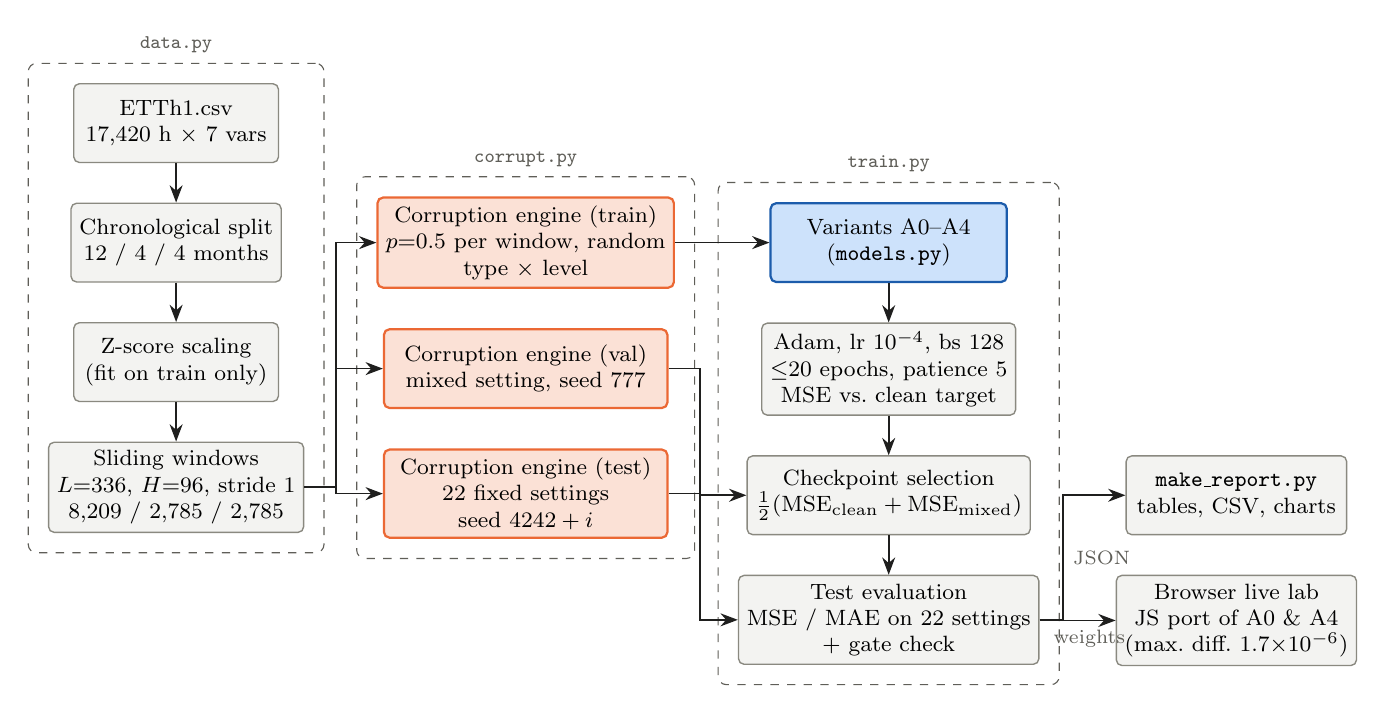
\begin{tikzpicture}[node distance=5mm and 6mm]
  \node[blk, minimum width=26mm] (csv) {ETTh1.csv\\17{,}420 h $\times$ 7 vars};
  \node[blk, minimum width=26mm, below=of csv] (split) {Chronological split\\12 / 4 / 4 months};
  \node[blk, minimum width=26mm, below=of split] (scale) {Z-score scaling\\(fit on train only)};
  \node[blk, minimum width=26mm, below=of scale] (win) {Sliding windows\\$L{=}336$, $H{=}96$, stride 1\\8{,}209 / 2{,}785 / 2{,}785};

  \node[accblk, minimum width=36mm, right=12mm of split] (ctrain) {Corruption engine (train)\\$p{=}0.5$ per window, random\\type $\times$ level};
  \node[accblk, minimum width=36mm, below=of ctrain] (cval) {Corruption engine (val)\\mixed setting, seed 777};
  \node[accblk, minimum width=36mm, below=of cval] (ctest) {Corruption engine (test)\\22 fixed settings\\seed $4242+i$};

  \node[newblk, minimum width=30mm, right=12mm of ctrain] (models) {Variants A0--A4\\(\texttt{models.py})};
  \node[blk, minimum width=30mm, below=of models] (train) {Adam, lr $10^{-4}$, bs 128\\$\le$20 epochs, patience 5\\MSE vs.\ clean target};
  \node[blk, minimum width=30mm, below=of train] (sel) {Checkpoint selection\\$\tfrac12(\text{MSE}_{\text{clean}}+\text{MSE}_{\text{mixed}})$};
  \node[blk, minimum width=30mm, below=of sel] (eval) {Test evaluation\\MSE / MAE on 22 settings\\+ gate check};

  \node[blk, minimum width=28mm, right=12mm of sel] (rep) {\texttt{make\_report.py}\\tables, CSV, charts};
  \node[blk, minimum width=28mm, below=of rep] (demo) {Browser live lab\\JS port of A0 \& A4\\(max.\ diff.\ $1.7{\times}10^{-6}$)};

  \draw[flow] (csv) -- (split);
  \draw[flow] (split) -- (scale);
  \draw[flow] (scale) -- (win);
  \draw[flow] (win.east) -- ++(4mm,0) |- (ctrain.west);
  \draw[flow] (win.east) -- ++(4mm,0) |- (cval.west);
  \draw[flow] (win.east) -- ++(4mm,0) |- (ctest.west);
  \draw[flow] (ctrain) -- (models);
  \draw[flow] (models) -- (train);
  \draw[flow] (train) -- (sel);
  \draw[flow] (cval.east) -- ++(4mm,0) |- (sel.west);
  \draw[flow] (sel) -- (eval);
  \draw[flow] (ctest.east) -- ++(4mm,0) |- (eval.west);
  \draw[flow] (eval.east) -- ++(3mm,0) |- (rep.west) node[pos=0.25, lbl, right] {JSON};
  \draw[flow] (eval.east) -- ++(3mm,0) |- (demo.west) node[pos=0.75, lbl, below] {weights};

  \begin{scope}[on background layer]
    \node[draw=muted, dashed, rounded corners=3pt, inner sep=2.5mm, fit=(csv)(win), label={[lbl]above:\texttt{data.py}}] {};
    \node[draw=muted, dashed, rounded corners=3pt, inner sep=2.5mm, fit=(ctrain)(ctest), label={[lbl]above:\texttt{corrupt.py}}] {};
    \node[draw=muted, dashed, rounded corners=3pt, inner sep=2.5mm, fit=(models)(eval), label={[lbl]above:\texttt{train.py}}] {};
  \end{scope}
\end{tikzpicture}
\end{document}
